% -*- latex -*-
%%%%%%%%%%%%%%%%%%%%%%%%%%%%%%%%%%%%%%%%%%%%%%%%%%%%%%%%%%%%%%%%
%%%%%%%%%%%%%%%%%%%%%%%%%%%%%%%%%%%%%%%%%%%%%%%%%%%%%%%%%%%%%%%%
%%%%
%%%% This text file is part of the source of 
%%%% `Introduction to High-Performance Scientific Computing'
%%%% by Victor Eijkhout, copyright 2012-2022
%%%%
%%%% This book is distributed under a Creative Commons Attribution 3.0
%%%% Unported (CC BY 3.0) license and made possible by funding from
%%%% The Saylor Foundation \url{http://www.saylor.org}.
%%%%
%%%%%%%%%%%%%%%%%%%%%%%%%%%%%%%%%%%%%%%%%%%%%%%%%%%%%%%%%%%%%%%%
%%%%%%%%%%%%%%%%%%%%%%%%%%%%%%%%%%%%%%%%%%%%%%%%%%%%%%%%%%%%%%%%

\lstset{language=CMake}

\begin{table}[p]
  \catcode`\_=12
  \begin{tabular}{>{\ttfamily}rp{3in}}
    \toprule
    \multicolumn{2}{c}{General directives}\\
    cmake_minimum_required     &specify minimum cmake version\\
    project                    &name and version number of this project\\
    install                    &specify directory where to install targets\\
    \midrule
    \multicolumn{2}{c}{Project building directives}\\
    add_executable             &specify executable name and source files for it\\
    add_library                &specify library name and files to go into it\\
    add_subdirectory           &specify subdirectory where cmake also needs to run\\
    target_link_libraries      &specify executable and libraries to link into it\\
    target_include_directories &specify include directories, privately or publicly\\
    find_package               &other package to use in this build\\
    \midrule
    \multicolumn{2}{c}{Utility stuff}\\
    target_compile_options     &literal options to include\\
    target_compile_features    &things that will be translated by cmake into options\\
    target_compile_definitions &macro definitions to be set private or publicly\\
    file                       &define macro as file list\\
    message                    &Diagnostic to print, subject to level specification\\
    \midrule
    \multicolumn{2}{c}{Control}\\
    if() else() endif()        &conditional\\
    \bottomrule
  \end{tabular}
  \caption{Cmake commands.}
  \label{tab:cmake-commands}
\end{table}

\Level 0 {CMake as build system}

\indexterm{CMake} is a general build system that uses other systems
such as \indexterm{Make} as a back-end.
The general workflow is:
\begin{enumerate}
\item The configuration stage. Here the \indextermtt{CMakeLists.txt} file
  is parsed, and \n{build} directory populated. This typically looks like:
\begin{verbatim}
mkdir build
cd build
cmake <source location>
\end{verbatim}
Some people create the build directory in the source tree,
in which case the cmake command is
\begin{verbatim}
cmake ..
\end{verbatim}
Other put the build directory next to the source, in which case:
\begin{verbatim}
cmake ../src_directory
\end{verbatim}
\item The build stage. Here the installation-specific compilation
  in the build directory is performed.
  With Make as the `generator' this would be
\begin{verbatim}
cd build
make
\end{verbatim}
but more generally
\begin{verbatim}
cmake --build <build directory>
\end{verbatim}
Alternatively, you could use generators such as \indexterm{ninja},
\indexterm{Visual Studio}, or \indexterm{XCode}:
\begin{verbatim}
cmake -G ninja
  ## the usual arguments
\end{verbatim}
\item The install stage. This can move binary files to a permanent
  location, such as putting library files in \n{/url/lib}:
\begin{verbatim}
make install
\end{verbatim}
or 
\begin{verbatim}
cmake --install <build directory>
\end{verbatim}
\end{enumerate}
The directory structure is illustrated in figure~\ref{fig:cmake-buildinstall}.


\makeatletter
%% from https://tex.stackexchange.com/a/34268/38308
\newcount\dirtree@lvl
\newcount\dirtree@plvl
\newcount\dirtree@clvl
\def\dirtree@growth{%
  \ifnum\tikznumberofcurrentchild=1\relax
  \global\advance\dirtree@plvl by 1
  \expandafter\xdef\csname dirtree@p@\the\dirtree@plvl\endcsname{\the\dirtree@lvl}
  \fi
  \global\advance\dirtree@lvl by 1\relax
  \dirtree@clvl=\dirtree@lvl
  \advance\dirtree@clvl by -\csname dirtree@p@\the\dirtree@plvl\endcsname
  \pgf@xa=1cm\relax
  \pgf@ya=-1cm\relax
  \pgf@ya=\dirtree@clvl\pgf@ya
  \pgftransformshift{\pgfqpoint{\the\pgf@xa}{\the\pgf@ya}}%
  \ifnum\tikznumberofcurrentchild=\tikznumberofchildren
  \global\advance\dirtree@plvl by -1
  \fi
}

\tikzset{
  dirtree/.style={
    growth function=\dirtree@growth,
    every node/.style={anchor=north},
    every child node/.style={anchor=west},
    edge from parent path={(\tikzparentnode\tikzparentanchor) |- (\tikzchildnode\tikzchildanchor)}
  }
}
\makeatother

\begin{figure}[ht]
  \hbox to \textwidth\bgroup
  \begin{minipage}{.45\textwidth}
    \tikzsetnextfilename{cmake-insource}
    \begin{tikzpicture}[dirtree]
      \node{dir}
      child { node {src} child { node {build} }
      }
      child { node {install} }
      ;
    \end{tikzpicture}
  \end{minipage}
  \hss
  \begin{minipage}{.45\textwidth}
    \tikzsetnextfilename{cmake-outsource}
    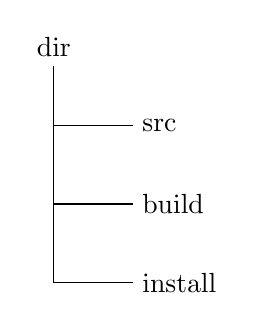
\begin{tikzpicture}[dirtree]
      \node{dir}
      child { node {src} }
      child { node {build} }
      child { node {install} }
      ;
    \end{tikzpicture}
  \end{minipage}
  \egroup
  \caption{In-source (left) and out-of-source (right) build schemes.}
  \label{fig:cmake-buildinstall}
\end{figure}

\Level 1 {Target philosophy}

Modern Cmake works through declaring targets and their requirements.
For requirements during building:
\begin{lstlisting}
target_some_requirement( the_target PRIVATE the require ments )
\end{lstlisting}
Usage requirements:
\begin{lstlisting}
target_some_requirement( the_target PUBLIC the require ments )
\end{lstlisting}

\Level 1 {Languages}

Cmake is largely aimed at~C++, but it easily supports C as well.
For \emph{Fortran}\index{CMake!Fortran support} support,
first to 
\begin{lstlisting}
enable_language(Fortran)
\end{lstlisting}
Note that capitalization: this also holds for all variables
such as \indexcmake{CMAKE_Fortran_COMPILER}.

\Level 1 {Script structure}

\begin{tabular}{lp{3in}}
  \toprule
  Commands learned in this section\\
  \midrule
  \lstinline+cmake_minimum_required+&declare minimum required version for this script\\
  \lstinline+project+&declare a name for this project\\
  \bottomrule
\end{tabular}

CMake is driven by the \indextermttdef{CMakeLists.txt} file.
This needs to be in the root directory of your project.
(You can additionally have files by that name in subdirectories.)

Since cmake has changed quite a bit over the years,
and is still evolving,
it is a good idea to start each script with a declaration
of the (minimum) required version:
\begin{lstlisting}
cmake_minimum_required( VERSION 3.12 )
\end{lstlisting}
You can query the version of your cmake executable:
\begin{verbatim}
$ cmake --version
cmake version 3.19.2
\end{verbatim}

You also need to declare a project name and version,
which need not correspond to any file names:
\begin{lstlisting}
project( myproject VERSION 1.0 )
\end{lstlisting}

\newpage
\Level 0 {Examples cases}

\Level 1 {Executable from sources}

\begin{tabular}{lp{3in}}
  \toprule
  Commands learned in this section\\
  \midrule
  \lstinline+add_executable+&declare an executable and its sources\\
  \lstinline+install+&indicate location where to install this project\\
  \lstinline+PROJECT_NAME+&macro that expands to the project name \\
  \bottomrule
\end{tabular}

\begin{floatingfigure}[r]{2.5in}
  \begin{minipage}{2.5in}
    \tikzsetnextfilename{cmake-install}
    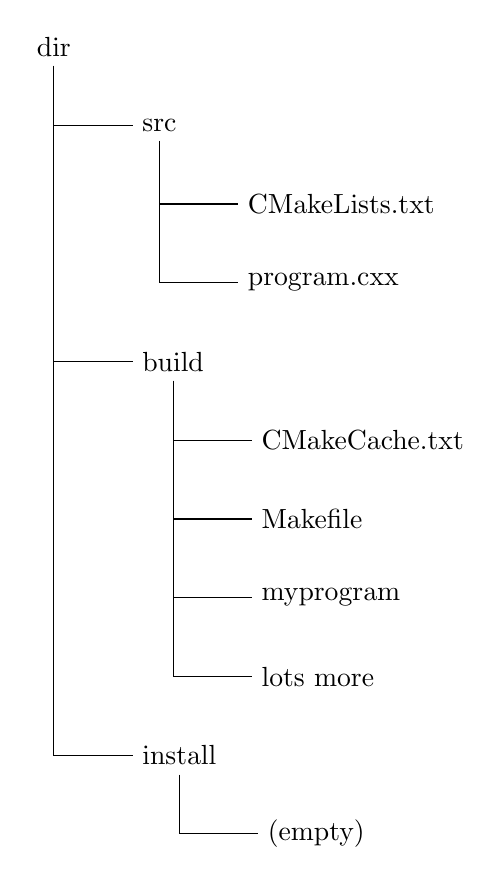
\begin{tikzpicture}[dirtree]
      \node{dir}
      child { node {src}
        child { node {CMakeLists.txt} }
        child { node {program.cxx} } }
      child { node {build}
        child { node {CMakeCache.txt} }
        child { node {Makefile} }
        child { node {myprogram} }
        child { node {lots more} } }
      child { node {install}
        child { node {(empty)} } }
      ;
    \end{tikzpicture}
  \end{minipage}
\end{floatingfigure}
%
If you have a project that is supposed to deliver an executable,
you declare in your \texttt{CMakeLists.txt}:
\begin{lstlisting}
add_executable( myprogram program.cxx )
\end{lstlisting}
Often, the name of the executable is the name of the project,
so you'd specify:
\begin{lstlisting}
add_executable( ${PROJECT_NAME} program.cxx )
\end{lstlisting}
%
In order to move the executable to the install location,
you need a clause
\begin{lstlisting}
install( TARGETS myprogram DESTINATION . )
\end{lstlisting}
Without the \indexcmake{DESTINATION} clause, a default \n{bin} directory
will be created; specifying \indexcmake{DESTINATION foo} will put the
program in a \n{foo} directory.

\begin{floatingfigure}[r]{2.5in}\vskip3in\end{floatingfigure}
%
In the figure on the right we have also indicated the \n{build} directory,
which from now on we will not show again.
It contains automatically generated files that are hard to
decyper.or debug. Yes, there is a \n{Makefile}, but even for simple
projects this is too complicated to debug by hand if your cmake
installation misbehaves.

Here is the full \n{CMakeLists.txt}:
%
\lstinputlisting{tutorials/cmake/single/CMakeLists.txt}

\newpage
\Level 1 {Making libraries}

\begin{tabular}{lp{3in}}
  \toprule
  Commands learned in this section\\
  \midrule
  \lstinline+add_library+&declare a library and its sources\\
  \lstinline+target_link_libraries+&indicate that the library belong with an executable\\
  \bottomrule
\end{tabular}

\begin{floatingfigure}[r]{2.5in}
  \begin{minipage}{2.5in}
    \tikzsetnextfilename{cmake-lib}
    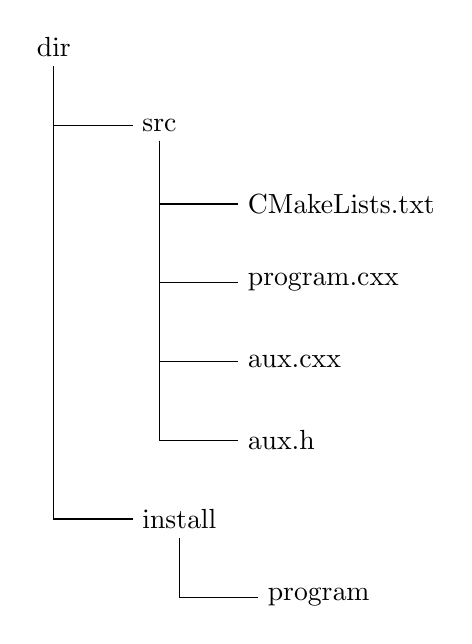
\begin{tikzpicture}[dirtree]
      \node{dir}
      child { node {src}
        child { node {CMakeLists.txt} }
        child { node {program.cxx} }
        child { node {aux.cxx} }
        child { node {aux.h} }
      }
      child { node {install}
        child { node {program} }
      }
      ;
    \end{tikzpicture}
%%       [dir [src [CMakeLists.txt] [program.cxx] [aux.cxx] [aux.h] ]
%%         [install [program] ] ]
  \end{minipage}
\end{floatingfigure}
%
If there is only one source file, this is all you need.
However, often you will build libraries.
You declare those with an \indexcmake{add_library} clause:
\begin{lstlisting}
add_library( auxlib aux.cxx aux.h )
\end{lstlisting}
Next, you need to link that library into the program:
\begin{lstlisting}
target_link_libraries( program PRIVATE auxlib )
\end{lstlisting}
The \indexcmake{PRIVATE} clause means that the library is only for
purposes of building the executable.
(Use \indexcmake{PUBLIC} to have the library be included in the installation;
we will explore that in the next section.)

The full \n{CMakeLists.txt}:
%
\lstinputlisting{tutorials/cmake/multiple/CMakeLists.txt}

Note that private shared libraries make no sense, as they will give
runtime unresolved references.

\Level 2 {Testing the generated makefiles}

In the Make tutorial \ref{tut:make} you learned how Make will only recompile
the strictly necessary files when a limited edit has been made.
The makefiles generated by CMake behave similarly.
With the structure above, we first touch the \n{aux.cxx} file,
which necessitates rebuilding the library:
%
\verbatiminput{tutorials/cmake/multiple-touch1.txt}

On the other hand, if we edit a header file, the main program
needs to be recompiled too:
%
\verbatiminput{tutorials/cmake/multiple-touch1.txt}

\newpage
\Level 1 {Finding subdirectories for the build}

\begin{tabular}{lp{3in}}
  \toprule
  Commands learned in this section\\
  \midrule
  \lstinline+target_include_directories+&indicate include directories needed\\
  \lstinline+target_sources+&specify more sources for a target\\
  \lstinline+CMAKE_CURRENT_SOURCE_DIR+&variable that expands to the current directory\\
  \lstinline+file+&define single-name synonym for multiple files\\
  \lstinline+GLOB+&define single-name synonym for multiple files\\
  \bottomrule
\end{tabular}

\begin{floatingfigure}[r]{2.5in}
  \begin{minipage}{2.5in}
    \tikzsetnextfilename{cmake-includedir}
    \begin{tikzpicture}[dirtree]
      \node{dir}
      child { node {src}
        child { node {CMakeLists.txt} }
        child { node {program.cxx} }
        child { node {src}
          child { node {aux.cxx} } }
        child { node {inc}
          child { node {aux.h} }
        }
      }
      child { node {install}
        child { node {program} }
      }
      ;
    \end{tikzpicture}
%%       [dir [src [CMakeLists.txt] [program.cxx]
%%           [src [aux.cxx] ]
%%           [inc [aux.h] ]
%%         [install [program] ] ] ]
  \end{minipage}
\end{floatingfigure}
%
If your program needs to be built using header files from a subdirectory,
meaning:
\begin{verbatim}
cc -c yourprogram.c -I./some/dir
\end{verbatim}
you can specify that include path with \indexcmake{target_include_directories}.
It is best to make such paths relative to
\indexcmake{CMAKE_CURRENT_SOURCE_DIR},
or the source root \indexcmake{CMAKE_SOURCE_DIR},
or equivalently \indexcmake{PROJECT_SOURCE_DIR}

\begin{floatingfigure}[r]{2.5in}\vskip3in\end{floatingfigure}
%
Usually, when you start making such directory structure,
you will also have sources in subdirectories.
If you only need to compile them into the main executable,
you could list them into a variable
\begin{lstlisting}
set( SOURCES program.cxx src/aux.cxx )
\end{lstlisting}
and use that variable.
However, this is deprecated practice;
it is recommended to use \indexcmake{target_sources}:
\begin{lstlisting}
target_sources( program PRIVATE src/aux1.cxx src/aux2.cxx )
\end{lstlisting}
Use of a wildcard is not trivial:
\begin{lstlisting}
file( GLOB AUX_FILES "src/*.cxx" )
target_sources( program PRIVATE ${AUX_FILES} )
\end{lstlisting}

Complete cmake file:
%
\lstinputlisting{tutorials/cmake/includedir/CMakeLists.txt}

\newpage
\Level 1 {Making a library}

\begin{tabular}{lp{3in}}
  \toprule
  Commands learned in this section\\
  \midrule
  \lstinline+add_library+&declare a library and its sources\\
  \lstinline+target_link_libraries+&declare a library to link into the target\\
  \lstinline+SHARED+&indicated to make shared libraries\\
  \bottomrule
\end{tabular}

\begin{floatingfigure}[r]{2.5in}
  \begin{minipage}{2.5in}
    \tikzsetnextfilename{cmake-withlib}
    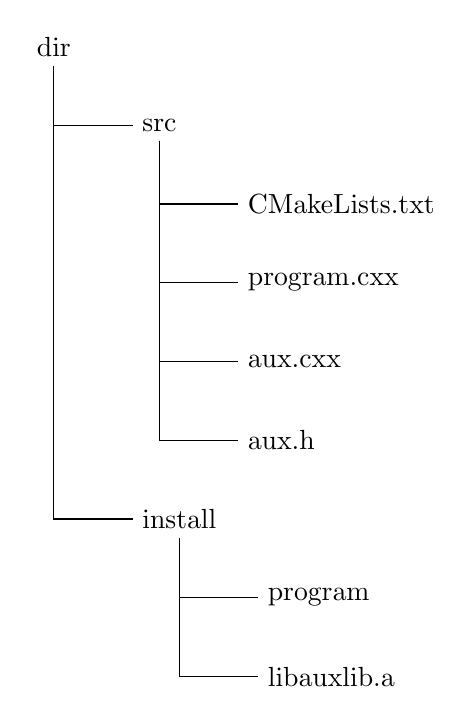
\begin{tikzpicture}[dirtree]
      \node{dir}
      child { node {src}
        child { node {CMakeLists.txt} }
        child { node {program.cxx} }
        child { node {aux.cxx} }
        child { node {aux.h} }
      }
      child { node {install}
        child { node {program} }
        child { node {libauxlib.a} }
      }
      ;
    \end{tikzpicture}
%%       [dir [src [CMakeLists.txt] [program.cxx] [aux.cxx] [aux.h] ]
%%         [install [program] [libauxlib.a] ] ]
  \end{minipage}
\end{floatingfigure}
%
In order to create a library we use \indexcmake{add_library},
and we link it into the target program with \indexcmake{target_link_libraries}.

By default the library is build as a static \texttt{.a} file,
but adding
\begin{lstlisting}
add_library( auxlib SHARED aux.cxx aux.h )
\end{lstlisting}
or adding a runtime flag
\begin{verbatim}
cmake -D BUILD_SHARED_LIBS=TRUE
\end{verbatim}
changes that to a shared \texttt{.so} type.

The full cmake file:
%
\lstinputlisting{tutorials/cmake/withlib/CMakeLists.txt}

\newpage
\Level 1 {Sub directories in the installation}
\label{sec:cmake-install-dirs}
\label{sec:cmake-rpath}

\begin{tabular}{lp{3in}}
  \toprule
  Commands learned in this section\\
  \midrule
  \lstinline+add_subdirectory+&declare a subdirectory where cmake needs to be run\\
  \lstinline+CMAKE_CURRENT_SOURCE_DIR+&directory where this command is evaluated\\
  \lstinline+CMAKE_CURRENT_BINARY_DIR+&\\
  \lstinline+LIBRARY_OUTPUT_PATH+&\\
  \lstinline+FILES_MATCHING PATTERN+&wildcard indicator\\
  \bottomrule
\end{tabular}

\begin{floatingfigure}[r]{2.5in}
  \begin{minipage}{2.5in}
    \tikzsetnextfilename{cmake-publiblib}
    \begin{tikzpicture}[dirtree]
      \node{dir}
      child { node {src}
        child { node {CMakeLists.txt} }
        child { node {program.cxx} }
        child { node {lib}
          child { node {CMakeLists.txt} }
          child { node {aux.cxx} }
          child { node {aux.h} }
        }
      }
      child { node {install}
        child { node {program} }
        child { node {lib}
          child { node {libauxlib.so} }
        }
      }
      ;
    \end{tikzpicture}
%%       [dir [src [CMakeLists.txt] [program.cxx]
%%           [lib [CMakeLists.txt] [aux.cxx] [aux.h] ]
%%         [install [program] [lib [libauxlib.so] ] ] ] ]
  \end{minipage}
\end{floatingfigure}
%
If your sources are spread over multiple directories,
there needs to be a \texttt{CMakeLists.txt} file in each,
and you need to declare the existence of those directories.
Let's start with the obvious choice of putting library files in a \n{lib} directory:
\begin{lstlisting}
add_subdirectory( lib )
\end{lstlisting}
For instance, a library directory would have a \n{CMakeLists.txt} file:
%
\lstinputlisting{tutorials/cmake/publiclib/lib/CMakeLists.txt}
%
to build the library file from the sources indicated,
and to install it in a \n{lib} subdirectory.

We also add a clause to install the header files in an include directory:
\begin{lstlisting}
install( FILES aux.h DESTINATION include )
\end{lstlisting}
For installing multiple files, use
\begin{lstlisting}
install(DIRECTORY ${CMAKE_CURRENT_BINARY_DIR}
    DESTINATION ${LIBRARY_OUTPUT_PATH}
    FILES_MATCHING PATTERN "*.h")
\end{lstlisting}

One problem is to tell the executable where to find the library.
For this we use the \indextermtt{rpath} mechanism.
By default, Cmake sets it so that the executable in the build location
can find the library.
If you use a non-trivial install prefix, the following lines work:
\begin{lstlisting}
set( CMAKE_INSTALL_RPATH "${CMAKE_INSTALL_PREFIX}/lib" )
set( CMAKE_INSTALL_RPATH_USE_LINK_PATH TRUE )
\end{lstlisting}
Note that these have to be specified before the target.

The whole file:
%
\lstinputlisting{tutorials/cmake/publiclib/CMakeLists.txt}

\Level 1 {Finding and using external packages}

If your program depends on other libraries, there is a variety of ways
to let cmake find them.

\Level 2 {Cmake commandline options}

You can indicate the location of your external library explicitly on the commandline;
see section~\ref{sec:cmake-doption} for the basics.

\begin{lstlisting}
cmake -D OTHERLIB_INC_DIR=/some/where/include
      -D OTHERLIB_LIB_DIR=/somewhere/lib
\end{lstlisting}

Example cmake file:
%
\lstinputlisting{tutorials/cmake/usepubliclib/CMakeLists.txt}

\Level 2 {Package finding through `find library' and `find package'}

%% https://izzys.casa/2020/12/how-to-find-packages-with-cmake-the-basics/

\begin{tabular}{lp{3in}}
  \toprule
  Commands learned in this section\\
  \midrule
  \lstinline+find_library+&find a library with a \n{FOOConfig.cmake} file\\
  \lstinline+CMAKE_PREFIX_PATH+&location for \n{FOOConfig.cmake} files\\
  \lstinline+find_package+&find a library with a \n{FindFOO} module\\
  \lstinline+CMAKE_MODULE_PATH+&location for \n{FindFOO} modules\\
  \bottomrule
\end{tabular}

The \indexcmake{find_package} command looks for files with
a name \n{FindXXX.cmake}, which are searched
on the \indexcmake{CMAKE_MODULE_PATH}.
Unfortunately, the working of \indexcmake{find_package}
depend somewhat on the specific package.
For instance, most packages set a variable \lstinline{FooFound}
that you can test
\begin{lstlisting}
find_package( Foo )
if ( FooFound )
    # do something
else()
    # throw an error
endif()
\end{lstlisting}

Some libraries come with a \n{FOOConfig.cmake} file,
which is searched on the \indexcmake{CMAKE_PREFIX_PATH}
through \indexcmake{find_library}.
If it is found, you can test the variable it is supposed to set:
\begin{lstlisting}
find_library( FOOLIB foo )
if (FOOLIB)
  target_link_libraries( myapp PRIVATE ${FOOLIB} )
else()
  # throw an error
endif()
\end{lstlisting}

\Level 2 {OpenMP}

\begin{lstlisting}
find_package(OpenMP)
if(OpenMP_C_FOUND) # or CXX
else()
	message( FATAL_ERROR "Could not find OpenMP" )
endif()
# for C:
add_executable( ${program} ${program}.c )
target_link_libraries( ${program} PUBLIC OpenMP::OpenMP_C )
# for C++:
add_executable( ${program} ${program}.cxx )
target_link_libraries( ${program} PUBLIC OpenMP::OpenMP_CXX)
# for Fortran
enable_language(Fortran)
# test: if( OpenMP_Fortran_FOUND )
add_executable( ${program} ${program}.F90 )
target_link_libraries( ${program} PUBLIC OpenMP::OpenMP_Fortran )
\end{lstlisting}

\Level 2 {MKL}

Intel compiler installations come with cmake support:
there is a file \n{MKLConfig.cmake}.

\lstinputlisting{tutorials/cmake/mklcmake/CMakeLists.txt}

\Level 1 {Use of other packages through `pkg config'}

These days, many package support the \indextermunix{pkgconfig} mechanism.
\begin{enumerate}
\item Suppose you have a library \n{mylib}, installed in \n{/opt/local/mylib}.
\item If \n{mylib} supports \n{pkgconfig}, there is most likely a path
  \n{/opt/local/mylib/lib/pkgconfig}, containing a file \n{mylib.pc}.
\item Add the path that contains the \indextermunix{.pc} file to the
  \indextermunix{PKG_CONFIG_PATH} environment variable.
\end{enumerate}
Cmake is now able to find \n{mylib}:
\begin{lstlisting}
find_package( PkgConfig REQUIRED )
pkg_check_modules( MYLIBRARY REQUIRED mylib )
\end{lstlisting}

This defines variables
\begin{verbatim}
MYLIBRARY_INCLUDE_DIRS
MYLIBRARY_LIBRARY_DIRS
MYLIBRARY_LIBRARIES
\end{verbatim}
which you can then use in the \indexcmake{target_include_directories}
command.

\Level 2 {Example with pkg config: fmtlib}

In the following example, we use the \indexterm{fmtlib}.
The main cmake file:
%
\lstinputlisting{tutorials/cmake/fmtlib/CMakeLists.txt}

We continue using the \indexterm{fmtlib} library,
but now the generated library also has references to this library,
so we use \lstinline+target_link_directories+ and \lstinline+target_link_library+.

Main file:
%
\lstinputlisting{tutorials/cmake/fmtliblib/CMakeLists.txt}

Library file:
%
\lstinputlisting{tutorials/cmake/fmtliblib/prolib/CMakeLists.txt}

\Level 2 {Common packages: MPI}

This cmake setup searches for \n{mpich.pc}:
%
\lstinputlisting{tutorials/cmake/mpiprog/CMakeLists.txt}

\Level 1 {Header-only libraries}

Use the \indexcmake{INTERFACE} keyword.

\Level 0 {Customizing the compilation process}

\begin{tabular}{lp{3in}}
  \toprule
  Commands learned in this section\\
  \midrule
  \lstinline+add_compile_options+&global compiler options\\
  \lstinline+target_compile_features+&compiler-independent specification of compile flags\\
  \lstinline+target_compile_definitions+&pre-processor flags\\
  \lstinline+option+&query commandline option\\
  \bottomrule
\end{tabular}

\Level 1 {Customizing the compiler}

It's probably a good idea to tell cmake explicitly what compiler you are using,
otherwise it may find some default gcc version that came with your system.
Use the variables \indexcmake{CMAKE_CXX_COMPILER}, \indexcmake{CMAKE_C_COMPILER},
\indexcmake{CMAKE_LINKER}.

\Level 1 {Global and target flags}

Most of the time, compile options should be associated with a target.
For instance, some file could need a higher or lower optimization level,
or a specific C++ standard.
In that case, use \indexcmake{target_compiler_features}.

Certain options may need to be global, in which case you use
\indexcmake{add_compile_options}. Example:
\begin{lstlisting}
## from https://youtu.be/eC9-iRN2b04?t=1548
if (MVSC)
    add_compile_options(/W3 /WX)
else()
    add_compile_options(-W -Wall -Werror)
endif()
\end{lstlisting}

\Level 2 {Universal flags}

Certain flags have a universal meaning, but compiler-dependent realization.
For instance, to specify the C++ standard:
\begin{lstlisting}
target_compile_features(arias_demo PRIVATE cxx_std_17)
\end{lstlisting}
The variable \indexcmake{CMAKE_CXX_COMPILE_FEATURES}
contains the list of all features you can set.

Optimization flags can be set by specifying the \indexcmake{CMAKE_BUILD_TYPE}:
\begin{itemize}
\item 
    \indexcmake{Debug} corresponds to the \n{-g} flag;
\item
    \indexcmake{Release} corresponds to \n{-O3 -DNDEBUG};
\item
    \indexcmake{MinSizeRel} corresponds to \n{-Os -DNDEBUG}
\item 
    \indexcmake{RelWithDebInfo} corresponds to \n{-O2 -g -DNDEBUG}.
\end{itemize}
This variable will often be set from the commandline:
\begin{verbatim}
cmake .. -DCMAKE_BUILD_TYPE=Release
\end{verbatim}

\Level 2 {Custom}

Set the variable
\indexcmake{CMAKE_CXX_FLAGS}
or
\indexcmake{CMAKE_C_FLAGS};
also
\indexcmake{CMAKE_LINKER_FLAGS}
(but see section~\ref{sec:cmake-rpath}
for the popular \indextermtt{rpath} options.)

\Level 1 {Macro definitions}

Cmake can provide macro definitions:
\begin{lstlisting}
target_compile_definitions
  ( programname PUBLIC
    HAVE_HELLO_LIB=1 )
\end{lstlisting}
and your source could test these:
\lstset{language=C}
\begin{lstlisting}
#ifdef HAVE_HELLO_LIB
#include "hello.h"
#endif
\end{lstlisting}
\lstset{language=CMake}

\Level 1 {Commandline options}
\label{sec:cmake-doption}

Commandline options to cmake:
\begin{verbatim}
cmake -DSOME_FLAG=somevalue
\end{verbatim}
(with an optional space after the \n{-D})
can be queried by the cmake script by the \indexcmake{option} command:
\begin{lstlisting}
option( SOME_FLAG "A flag that has some function" defaultvalue )
\end{lstlisting}

\Level 0 {CMake scripting}
\label{sec:cmake-script}

\begin{tabular}{lp{3in}}
  \toprule
  Commands learned in this section\\
  \midrule
  \lstinline+option+&query a commandline option\\
  \lstinline+message+&trace message during cmake-ing\\
  \lstinline+set+&set the value of a variable\\
  \lstinline+CMAKE_SYSTEM_NAME+&variable containing the operating system name\\
  \bottomrule
\end{tabular}

The \indextermtt{CMakeLists.txt} file is a script,
though it doesn't much look like it.
\begin{itemize}
\item
  Instructions consist of a command, followed by a parenthesized
  list of arguments.
\item
  (All arguments are strings: there are no numbers.)
\item
  Each command needs to start on a new line, but otherwise
  whitespace and line breaks are ignored.
\end{itemize}

Comments start with a hash character.

\Level 1 {System dependencies}

\begin{lstlisting}
if (CMAKE_SYSTEM_NAME STREQUALS "Window")
  target_compile_options( myapp PRIVATE /W4 )
elseif (CMAKE_SYSTEM_NAME STREQUALS -Wall -Wextra -Wpedantic)
  target_compile_options( myapp PRIVATE /W4 )
endif()
\end{lstlisting}

\Level 1 {Messages, errors, and tracing}

The \indexcmake{message} command can be used to write output
to the console. This command has two arguments:
\begin{lstlisting}
message( STATUS "We are rolling!")
\end{lstlisting}
Instead of \indexcmake{STATUS} you can specify other logging levels
(this parameter is actually called `mode' in the documentation);
running for instance
\begin{verbatim}
cmake --log-level=NOTICE
\end{verbatim}
will display only messages of `notice' status or higher.

The possibilities here are: \indexcmake{FATAL_ERROR}, \indexcmake{SEND_ERROR},
\indexcmake{WARNING}, \indexcmake{AUTHOR_WARNING}, \indexcmake{DEPRECATION}, \indexcmake{NOTICE},
\indexcmake{STATUS}, \indexcmake{VERBOSE}, \indexcmake{DEBUG}, \indexcmake{TRACE}.

The \indexcmake{NOTICE}, \indexcmake{VERBOSE}, \indexcmake{DEBUG}, \indexcmake{TRACE} options
were added in \cmakestandard{3.15}.

For a complete trace of everything Cmake does, use
the commandline option \n{--trace}.

You can get a verbose make file by using the option
\begin{verbatim}
-D CMAKE_VERBOSE_MAKEFILE=ON
\end{verbatim}
on the cmake invocation. You still need \n{make V=1}.

\Level 1 {Variables}

Variables are set with \texttt{set},
or can be given on the commandline:
\begin{lstlisting}
cmake -D MYVAR=myvalue
\end{lstlisting}
Using the variable by itself gives the value,
except in strings, where a shell-like notation is needed:
\begin{lstlisting}
set(SOME_ERROR "An error has occurred")
message(STATUS "${SOME_ERROR}")
set(MY_VARIABLE "This is a variable")
message(STATUS "Variable MY_VARIABLE has value ${MY_VARIABLE}")
\end{lstlisting}

Some variables are set by other commands.
For instance the \texttt{project} command sets
\indextermtt{PROJECT_NAME} and \indextermtt{PROJECT_VERSION}.

Environment variables can be queried with the \indexcmake{ENV} command:
\begin{lstlisting}
set( MYDIR $ENV{MYDIR} )
\end{lstlisting}

\Level 2 {Numerical variables}

\begin{lstlisting}
math( EXPR lhs_var "math expr" )
\end{lstlisting}

\Level 1 {Control structures}

\Level 2 {Conditionals}

\begin{lstlisting}
if ( MYVAR MATCHES "value$" )
    message( NOTICE "Variable ended in 'value'" )
elseif( stuff )
    message( stuff )
else()
    message( NOTICE "Variable was otherwise" )
endif()
\end{lstlisting}

\Level 2 {Looping}

\begin{lstlisting}
while( myvalue LESS 50 )
    message( stuff )
endwhile()
\end{lstlisting}

\begin{lstlisting}
foreach ( var IN ITEMS item1 item2 item3 )
  ## something wityh ${var}
endforeach()
foreach ( var IN LISTS list1 list2 list3 )
  ## something wityh ${var}
endforeach()
\end{lstlisting}

Integer range, with inclusive bounds, upper bound zero by default:
\begin{lstlisting}
foreach ( idx RANGE 10 )
foreach ( idx RANGE 5 10 )
foreach ( idx RANGE 5 10 2 )
endforeach()
\end{lstlisting}

\Level 2 {Things not to do}

Do not use macros that affect all targets: \indexcmake{include_directories},
\indexcmake{add_definitions}, \indexcmake{link_libraries}.

Do not use \indexcmake{target_include_directories} outside your project:
that should be found through some of the above mechanisms.

\Level 2 {All the reasons I do not like the Professional Cmake book}

\begin{enumerate}
\item The \n{make install} idiom which I encounter in 100 percent of packages is not discussed.
\item The use of \lstinline{option} with commandline option is not discussed,
  in fact the term `commandline' does not even appear in the index.
\item Does not mention \n{cmake --build}.
\end{enumerate}
% LocalWords:  Eijkhout CMake workflow CMakeLists txt cmake mylibrary
% LocalWords:  programmain libsource libheader lib hellolibdir
